% fig5_dag.tex — practice as a confounder of the emotion-performance path
% Compile: xelatex fig5_dag.tex  ->  move fig5_dag.pdf to figure/
\documentclass[tikz,border=8pt]{standalone}
\usepackage{fontspec}
\setmainfont{Times New Roman}
\usetikzlibrary{positioning,arrows.meta}

\begin{document}
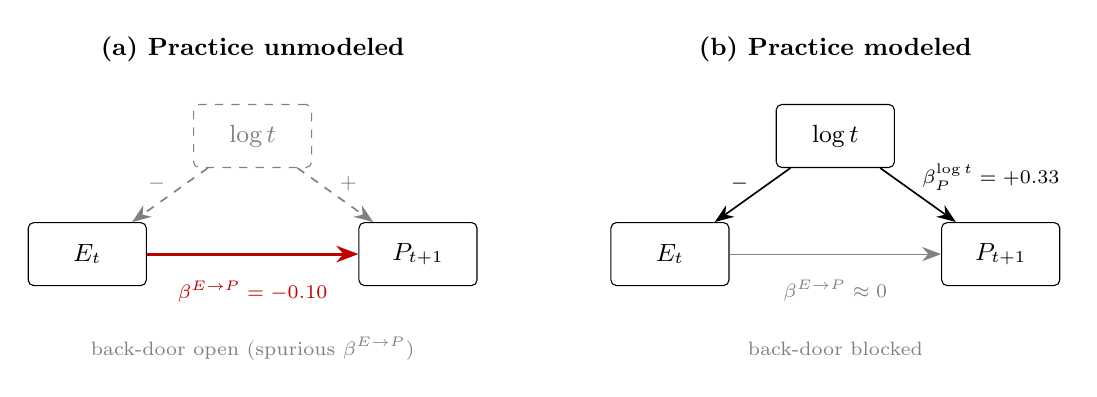
\begin{tikzpicture}[
  var/.style  = {draw, rounded corners=2pt, minimum width=15mm, minimum height=8mm, font=\small},
  ghost/.style= {draw, dashed, gray, rounded corners=2pt, minimum width=15mm, minimum height=8mm, font=\small\color{gray}},
  lab/.style  = {font=\scriptsize},
  arr/.style  = {-{Stealth[length=2.4mm]}, semithick},
  gharr/.style= {-{Stealth[length=2.4mm]}, semithick, gray, dashed},
  hot/.style  = {-{Stealth[length=2.8mm]}, line width=1.1pt, red!75!black},
  cold/.style = {-{Stealth[length=2.4mm]}, gray},
  panel/.style= {font=\small\bfseries}
]

% ================= Panel (a): practice unmodeled =================
\begin{scope}
  \node[panel] at (21mm,26mm) {(a) Practice unmodeled};
  \node[ghost] (T)  at (21mm,15mm) {$\log t$};
  \node[var]   (E)  at (0,0)       {$E_t$};
  \node[var]   (P)  at (42mm,0)    {$P_{t+1}$};

  \draw[gharr] (T) -- node[lab, above left=-1mm, gray]{$-$} (E);
  \draw[gharr] (T) -- node[lab, above right=-1mm, gray]{$+$} (P);
  \draw[hot]   (E) -- node[lab, below=2mm]{$\beta^{E\to P}=-0.10$} (P);
  \node[lab, gray, align=center] at (21mm,-12mm) {back-door open (spurious $\beta^{E\to P}$)};
\end{scope}

% ================= Panel (b): practice modeled =================
\begin{scope}[xshift=74mm]
  \node[panel] at (21mm,26mm) {(b) Practice modeled};
  \node[var]   (T2) at (21mm,15mm) {$\log t$};
  \node[var]   (E2) at (0,0)       {$E_t$};
  \node[var]   (P2) at (42mm,0)    {$P_{t+1}$};

  \draw[arr]  (T2) -- node[lab, above left=-1mm]{$-$} (E2);
  \draw[arr]  (T2) -- node[lab, above right=-1mm]{$\beta^{\log t}_{P}=+0.33$} (P2);
  \draw[cold] (E2) -- node[lab, below=2mm]{$\beta^{E\to P}\approx 0$} (P2);
  \node[lab, gray, align=center] at (21mm,-12mm) {back-door blocked};
\end{scope}

\end{tikzpicture}
\end{document}
